\section{Introduction}


\begin{frame}
   \frametitle{Pattern Recognition in Erlangen}

   \begin{center}
      \begin{tabular}{x{3cm} x{3cm} x{3cm}}
         \includegraphics[height=2.7cm]{\pngdir/niemann_frei.\png}   &
         \includegraphics[height=2.7cm]{\pngdir/Hornegger_frei.\png} &
         \includegraphics[height=2.7cm]{\pngdir/stefan_frei_bw.\png}   \\
         \tiny Prof.\ Dr.\ Heinrich Niemann                          &
         \tiny Prof.\ Dr.\ Joachim Hornegger                         &
         \tiny PD\ Dr.\ Stefan Steidl                                  \\
      \end{tabular}
   \end{center}
\end{frame}


\subsection{Topics of the Lecture}

\begin{frame}
   \frametitle{Lecture Topics}

   \vspace{-0.5cm}
   \begin{center}
      \resizebox{\linewidth}{!}{
         \alt<3->{
            \input{\texfigdir/classification3.pstex_t}
         }{\alt<2>{
               \input{\texfigdir/classification2.pstex_t}
            }{
               \input{\texfigdir/classification1.pstex_t}
            }}
      }
   \end{center}
\end{frame}

\ifnosummary
   \begin{frame}
      \frametitle{Lecture Topics}

      \begin{columns}
         \column{.4\linewidth}
         \begin{itemize}
            \item Bayes
            \item Na\"ive Bayes
            \item Logistic Regression
            \item Discriminant Analysis
            \item Perceptrons
            \item Support Vector Machines
         \end{itemize}

         \column{.5\linewidth}
         \begin{itemize}
            \item Norms
            \item Optimization
            \item Kernel Methods
            \item Expectation Maximization
            \item Ada Boost
            \item[]
         \end{itemize}
      \end{columns}
   \end{frame}


   \begin{frame}
      \frametitle{Pattern Recognition -- What For?}

      \begin{itemize}
         \item Speech recognition
         \item Image processing
         \item Fingerprint identification
         \item Optical character recognition (OCR)
         \item Industrial workflows
           \begin{itemize}
              \item Quality control
              \item Sorting
           \end{itemize}
         \item \ldots
      \end{itemize}
   \end{frame}

\fi

\subsection{Example: Iris Flower Classification}

\begin{frame}
   \frametitle{Example}

   \begin{itemize}
      \item ``Determining Iris flower according to species \\
        using optical sensing''
        \newline
        \begin{figure}
           \copyrightbox[b]{
              \makebox[.8\linewidth]{
                 \includegraphics[width=.8\linewidth]{\pngdir/sorting.\png}
              }
           }{1. Fisher 36, "The use of multiple measurements in taxonomic problems". \newline
              2. Anderson 36, "The species problem in Iris". Annals of the Missouri Botanical Garden.}
        \end{figure}

        \spread{}
      \item Risk:
        They may be sold interchangeably which annoys customers!
   \end{itemize}
\end{frame}

\begin{frame}
   \frametitle{Example \cont}
   \begin{figure}
      \copyrightbox[b]{
         \makebox[.8\linewidth]{
            \includegraphics[width=.8\linewidth]{\pngdir/1280px-Mature_flower_diagram.\png}
         }
      }{ \href{https://commons.wikimedia.org/wiki/File:Mature_flower_diagram.svg} {LadyofHats}, Public domain, via Wikimedia Commons}
   \end{figure}
\end{frame}


\begin{frame}
   \frametitle{Example \cont}

   \structure{Problem analysis}

   \begin{itemize}
      \item Set up a camera and take some sample images
      \item Extract characteristics that make distinction between species possible
        \begin{itemize}
           \item Sepal Length
           \item Sepal Width
           \item Petal Length
           \item Petal Width
           \item Color, etc.
        \end{itemize}
      \item The is the set of all suggested \structure{features} to explore for use in our classifier!
   \end{itemize}
\end{frame}


\begin{frame}
   \frametitle{Example \cont}

   \begin{itemize}
      \item \structure{Preprocessing}
        \begin{itemize}
           \item Segmentation operation: isolate flowers from one another and from the background\\[.5cm]
        \end{itemize}
      \item \structure{Feature extraction:} extract best features from single flower image
        \begin{itemize}
           \item Data reduction
           \item Curse of dimensionality\\[.5cm]
        \end{itemize}
      \item \structure{Classification} Classify features with a trained classifier
   \end{itemize}
\end{frame}


\begin{frame}
   \frametitle{Example \cont}

   \structure{Classification}

   \begin{itemize}
      \item Possible feature for discrimination: \structure{Sepal Length}
   \end{itemize}
   %      
   \begin{center}
      \includegraphics[width=.75\linewidth, trim={0  0.9cm 0 0},clip]{\pngdir/sepallength1.\png}\newline%
      \scriptsize{Sepal length in cm}\hspace{1.5cm}$\quad$
   \end{center}
   %    
   \begin{itemize}
      \item The sepal length alone is a \structure{poor feature} for classification!
   \end{itemize}
\end{frame}


\begin{frame}
   \frametitle{Example \cont}

   \begin{itemize}
      \setlength\itemsep{0.1cm}
      \item Another possible feature: \structure{Sepal Width}

        \begin{center}
           \includegraphics[width=.75\linewidth, trim={0  1.4cm 0 0.3cm},clip]{\pngdir/width.\png}\newline%
           \scriptsize{Sepal width in cm}\hspace{1.5cm}$\quad$
        \end{center}

      \item Relationship between \structure{decision boundary} and \structure{costs}!
      \item  What is worse?
        \begin{itemize}
           \item Red flowers in the blue bucket? $\Rightarrow$ Lower decision boundary!
           \item Blue flowers in the red bucket? $\Rightarrow$ Raise decision boundary!
        \end{itemize}
      \item Optimum decision always depends on definition of cost function
   \end{itemize}
\end{frame}


\begin{frame}
   \frametitle{Example \cont}

   \begin{itemize}
      \item Adopt \structure{Length} ($x_1$) and add the \structure{Width} ($x_2$) of the Sepal of the flower
   \end{itemize}

   \begin{displaymath}
      \mathsf{Flower} \longrightarrow \vec{x}^T = [x_1, x_2]
   \end{displaymath}

   \begin{center}
      \includegraphics[width=.65\linewidth]{\pngdir/irislinear.\png}
   \end{center}
\end{frame}


\begin{frame}
   \frametitle{Example \cont}

   \begin{itemize}
      \item We might add other features that are not correlated with the ones \\
        we already have.
        A precaution should be taken not to reduce the \\
        performance by adding such ``noisy features''.
      \item Ideally, the best decision boundary should be the one which provides an \structure{optimal performance} such as in the following figure:
   \end{itemize}

   \begin{center}
      \includegraphics[width=.65\linewidth]{\pngdir/irisoverfit.\png}
   \end{center}
\end{frame}


\begin{frame}
   \frametitle{Example \cont}

   \begin{itemize}
      \item However, our satisfaction is premature because the central aim of designing a classifier is to correctly classify \structure{novel} input.\\[.3cm]
      \item Issue of \structure{generalization}!
   \end{itemize}

   \begin{center}
      \includegraphics[width=.65\linewidth]{\pngdir/irisgeneral.\png}
   \end{center}
\end{frame}


\subsection{Pattern Recognition Task}

\begin{frame}
   \frametitle{Feature Extraction}

   \begin{itemize}
      \item Recorded input signal
        \begin{itemize}
           \item Camera, microphone, x-ray signal, etc. \\[.5cm]
        \end{itemize}
      \item Digitization: sampling and quantization
      \item Preprocessing
      \item Computation of features
   \end{itemize}
\end{frame}

{
\usebackgroundtemplate{\includegraphics[width=\paperwidth]{png/nextTime.png}}
\begin{frame}[plain]
\end{frame}
}


\begin{frame}
   \frametitle{Postulates for Pattern Recognition}

   \structure{6 Postulates:} \\[.5cm]

   \begin{enumerate}
      \item Availability of a \structure{representative sample} $\omega$ of \structure{patterns} ${}^i\vec{f}(\vec{x})$ \\
        for the given field of problems $\Omega$
        \begin{displaymath}
           \omega = \{{}^1\vec{f}(\vec{x}),\ldots,{}^N\vec{f}(\vec{x})\} \subseteq \Omega
        \end{displaymath}
        %      \vspace{.3cm}
        \pause

      \item A (simple) pattern has \structure{features}, which characterize \\
        its membership in a certain class $\Omega_\kappa$.
   \end{enumerate}
\end{frame}


\begin{frame}
   \frametitle{Postulates for Pattern Recognition \cont}

   \begin{enumerate}
      \setcounter{enumi}{2}
      \item Compact domain in the feature space of features of the same class; domains of different classes are (reasonably) separable.
        \begin{itemize}
           \item small \structure{intra-class distance}
           \item high \structure{inter-class distance} \\[.5cm]
        \end{itemize}
      \item[] Example of an increasingly less compact domain in the feature space:
   \end{enumerate}

   \begin{center}
      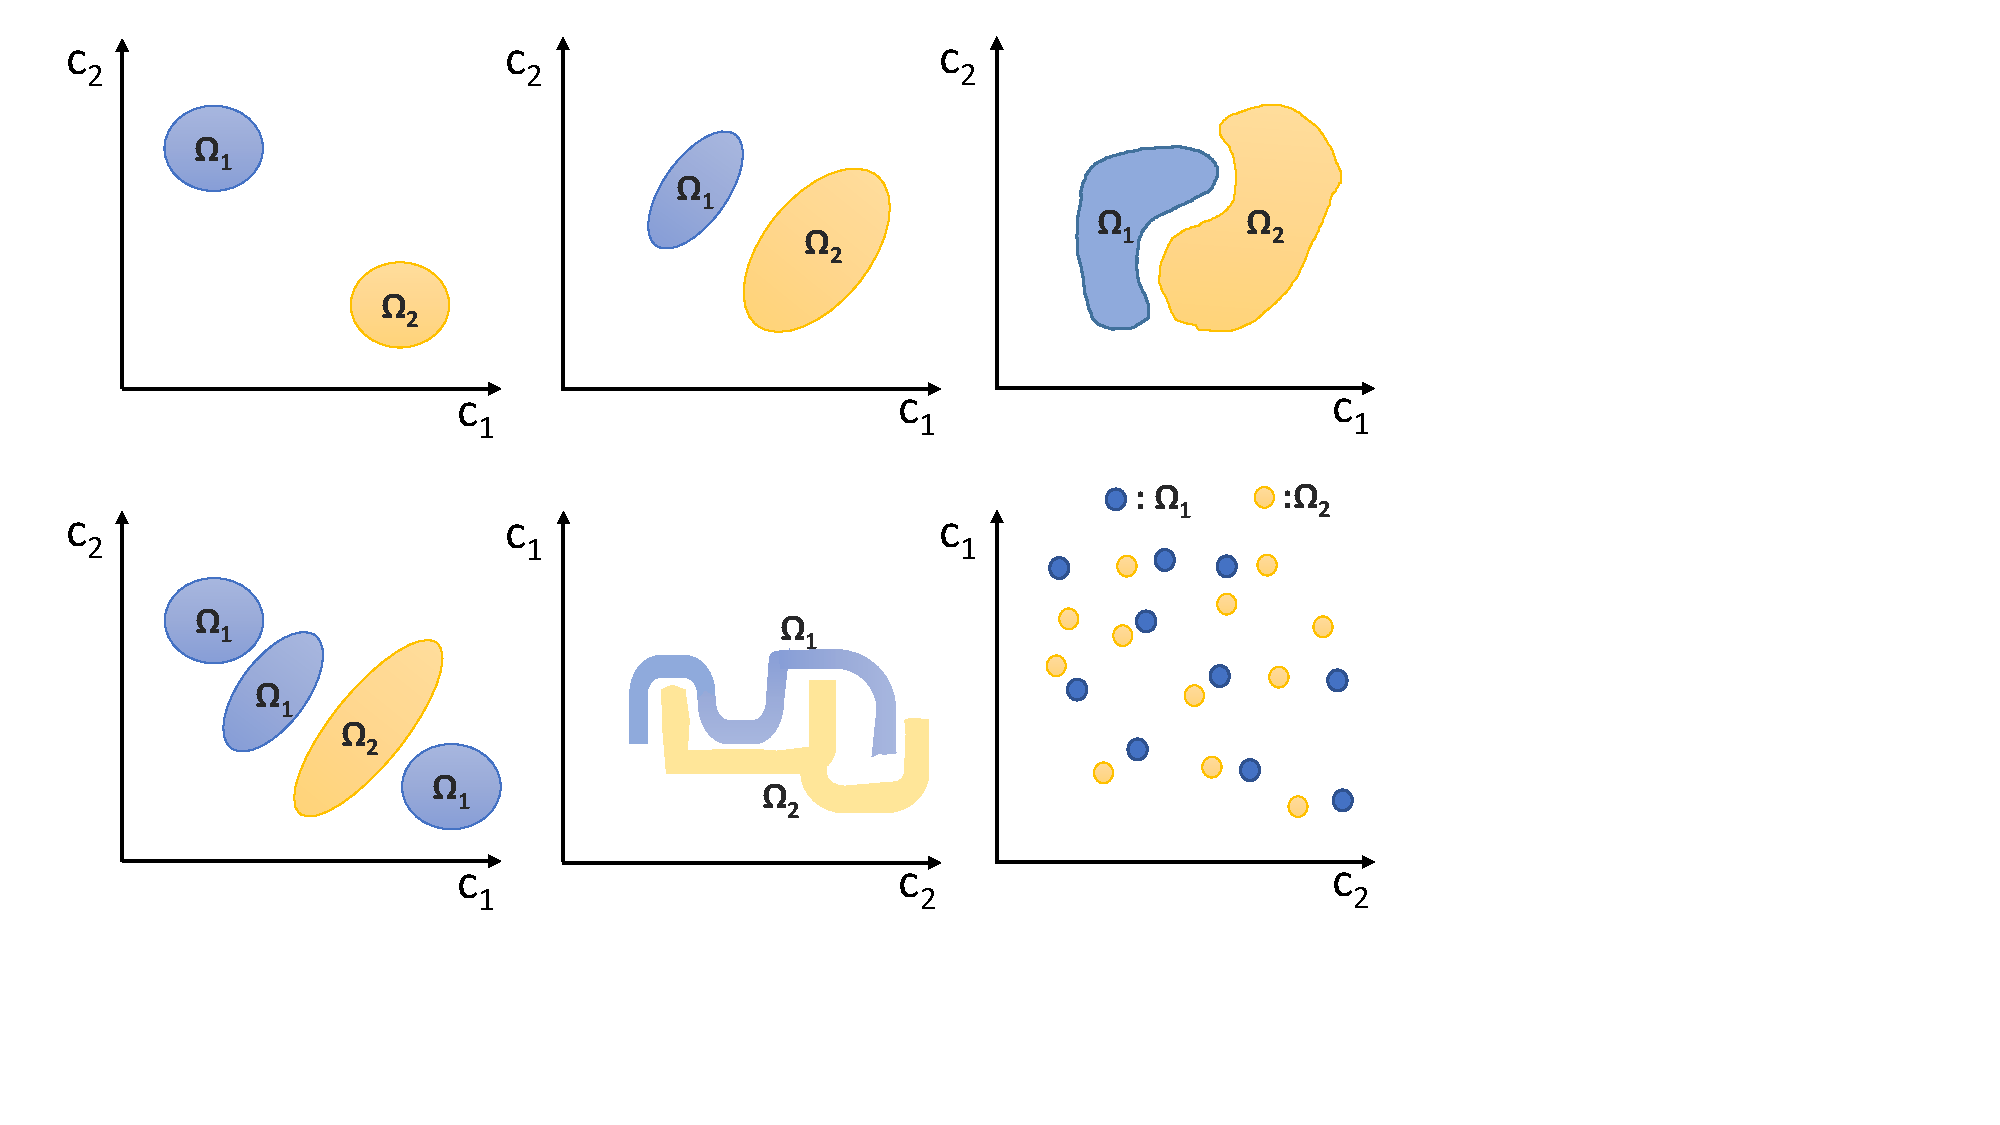
\includegraphics[width=.70\linewidth, trim={0  3cm 7cm 0cm},clip]{images/featurespace.pdf}
   \end{center}
\end{frame}


\begin{frame}
   \frametitle{Postulates for Pattern Recognition \cont}

   \begin{enumerate}
      \setcounter{enumi}{3}
      \item A (complex) pattern consists of \structure{simpler constituents}, which have certain relations to each other. A pattern may be decomposed into these constituents.\\[.3cm]
        \pause
      \item A (complex) pattern $\vec{f}(\vec{x}) \in \Omega$ has a certain \structure{structure}.
        Not any arrangement of simple constituents is a valid pattern. Many patterns may be represented with relatively few constituents.
   \end{enumerate}

   \begin{center}
      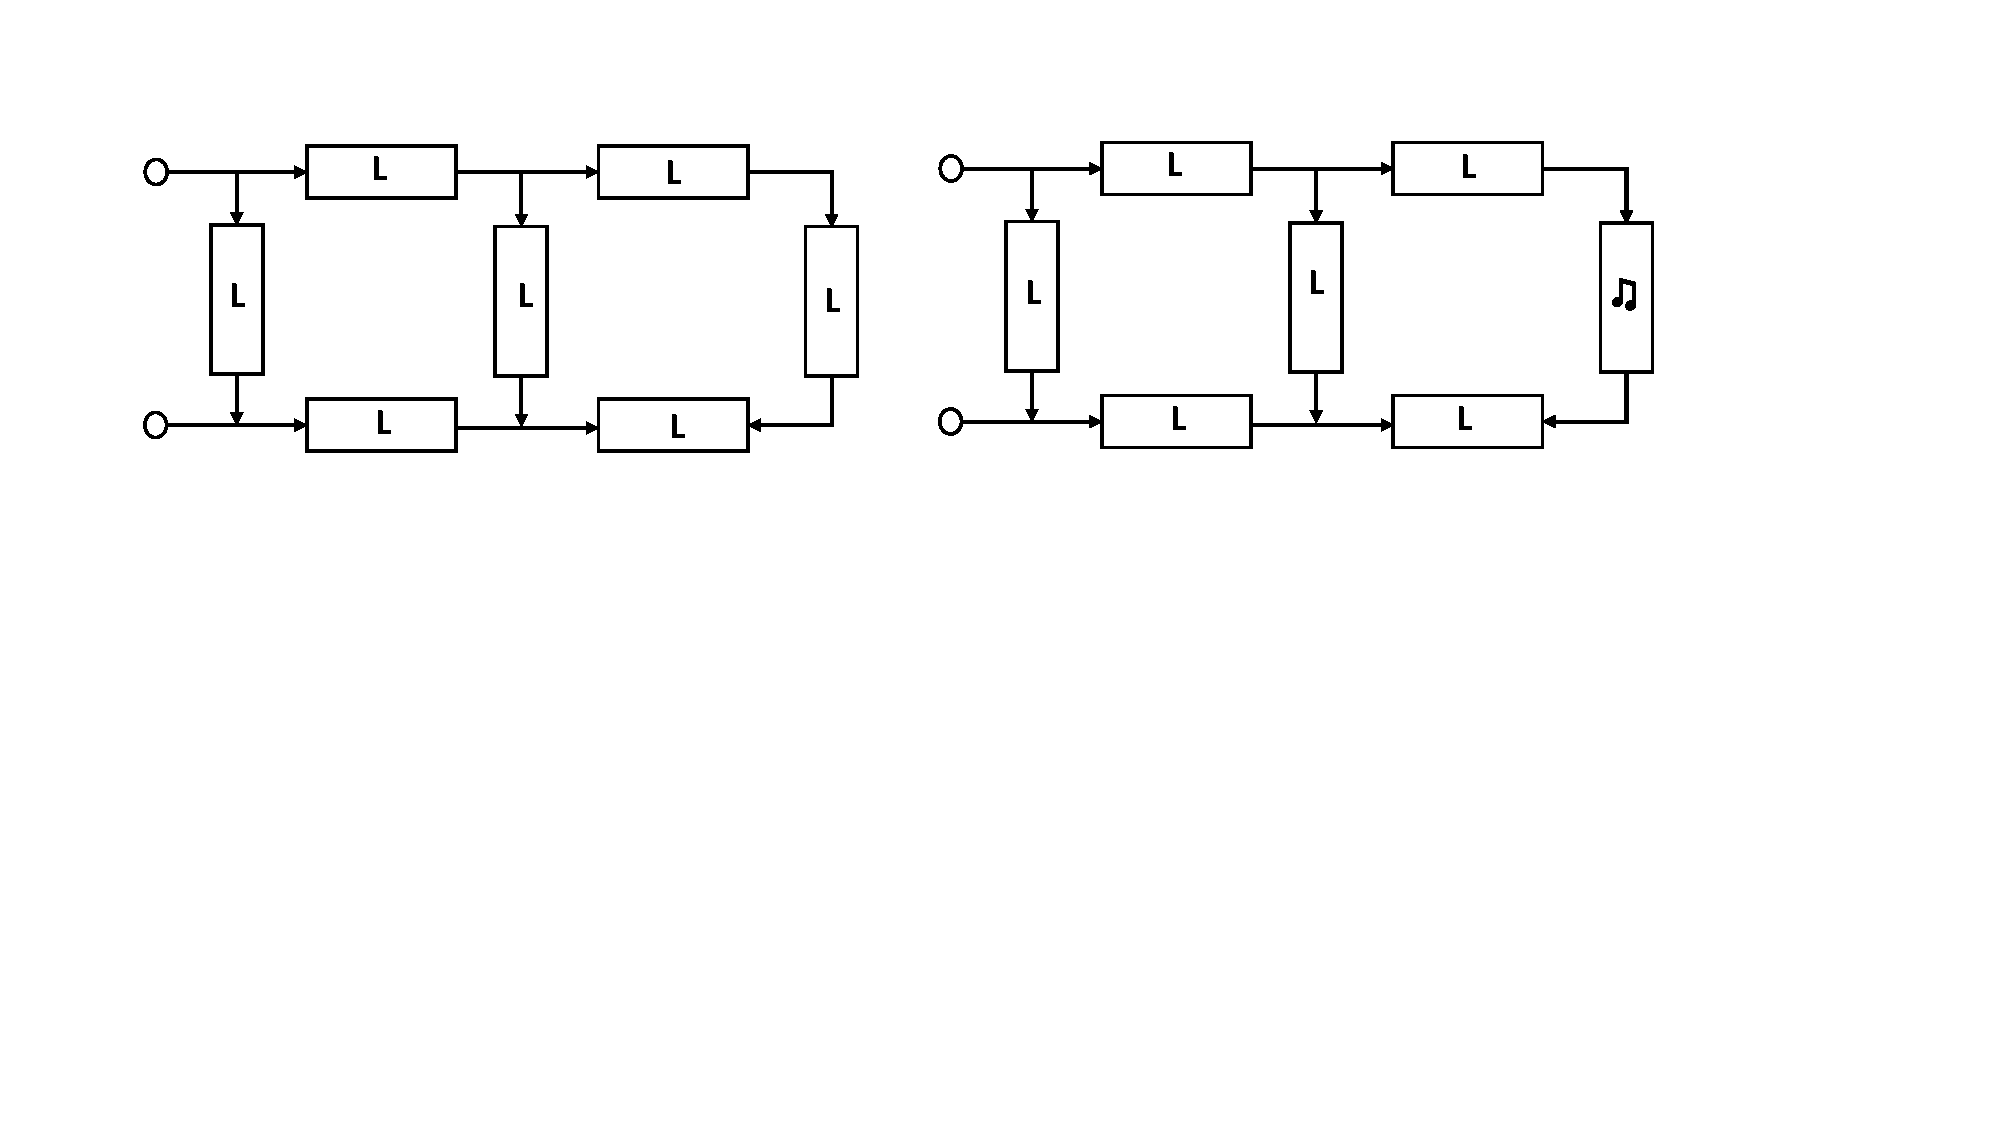
\includegraphics[width=\linewidth, trim={2cm 10cm 5cm 0cm},clip]{images/circuit.pdf}
   \end{center}
\end{frame}


\begin{frame}
   \frametitle{Postulates for Pattern Recognition \cont}

   \begin{enumerate}
      \setcounter{enumi}{5}
      \item Two patterns are \structure{similar} if their features or simpler constituents differ only lightly.
   \end{enumerate}
\end{frame}


\begin{frame}[fragile]
   \frametitle{Performance Evaluation}

   \begin{itemize}
      \item Feature vectors are used as input for the classifier
      \item Classifaction results in a discrete class index
      \item Confusion matrix:
   \end{itemize}

   \begin{table}
      \centering
      \small
      \newcommand{\C}[1]{$\Omega_{#1}$}
      \newcommand{\cc}[1]{$n_{#1}$}
      \newcommand{\CC}[1]{\multicolumn{1}{>{\columncolor[rgb]{0.8,0.8,0.8}}c}{\cc{#1}}}
      \begin{tabular}{c c | c c c c c | c}
          & \multicolumn{7}{c}{\structure{hypothesis}}                                                                            \\
          &                                            & \C{1}                 & \C{2}   & \C{3}   & \ldots   & \C{K}   & $\sum$  \\
         \cline{2-8}
         \multirow{5}{*}{\rotatebox{90}{\structure{reference}~~}}
          & \C{1}                                      & \CC{11}               & \cc{12} & \cc{13} & \ldots   & \cc{1K} & $N_{1}$ \\
          & \C{2}                                      & \cc{21}               & \CC{22} & \cc{23} & \ldots   & \cc{2K} & $N_{2}$ \\
          & \C{3}                                      & \cc{31}               & \cc{32} & \CC{33} & \ldots   & \cc{3K} & $N_{3}$ \\
          & \vdots                                     & \vdots                & \vdots  & \vdots  & $\ddots$ & \vdots  & \vdots  \\
          & \C{K}                                      & \cc{K1}               & \cc{K2} & \cc{K3} & \ldots   & \CC{KK} & $N_{K}$ \\
         \cline{2-8}
          & $\sum$                                     & \multicolumn{5}{c|}{} & $N$                                              \\
      \end{tabular}
      \caption{Confusion matrix with absolute frequencies for a $K$-class problem}
   \end{table}
\end{frame}


\begin{frame}[fragile]
   \frametitle{Performance Evaluation \cont}

   \structure{Evaluation of classifiers}

   \begin{itemize}
      \item Accuracy\,/\,Recognition Rate
           {\small
              \begin{displaymath}
                 \mathsf{RR} := \frac{1}{N} \sum_{\kappa=1}^{K}n_{\kappa\kappa} \cdot 100\,\%
              \end{displaymath}
              \pause
           }
      \item Recall and Precision
           {\small
              \begin{eqnarray*}
                 \mathsf{recall}_\kappa    & = & \frac{n_{\kappa\kappa}}{\sum_{i=1}^K n_{\kappa i}}
                 = \frac{n_{\kappa\kappa}}{N_\kappa} \\
                 \mathsf{precision}_\kappa & = & \frac{n_{\kappa\kappa}}{\sum_{i=1}^K n_{i \kappa}}
              \end{eqnarray*}
              \pause
           }
      \item (Unweighted) Average Recall
           {\small
              \begin{displaymath}
                 \mathsf{UAR} := \frac{1}{K} \sum_{\kappa=1}^K \frac{n_{\kappa\kappa}}{N_\kappa} \cdot 100\,\%
              \end{displaymath}
           }
   \end{itemize}
\end{frame}


\begin{frame}[fragile]
   \frametitle{Performance Evaluation \cont}

   \structure{Special case: only 2 classes}

   \begin{table}
      \centering
      \small
      \begin{tabular}{c c | c c |}
          & \multicolumn{1}{c}{}  & \multicolumn{2}{c}{\structure{Reference}}                         \\
          &                       & {\color{gr3}Positive}                     & {\color{gr3}Negative} \\
         \cline{2-4}
         \multirow{2}{*}{\rotatebox{90}{\structure{Hyp.}}}
          & {\color{gr3}Positive} & True Positive                             & False Positive        \\
          & {\color{gr3}Negative} & False Negative                            & True Negative         \\
         \cline{2-4}
      \end{tabular}
   \end{table}
   \spread

   \structure{Various performance measures:}

   \begin{itemize}
      \item True positive rate (hit rate, \structure{recall}, \structure{sensitivity}): $\frac{\#\mathsf{TP}}{\#\mathsf{TP} + \#\mathsf{FN}}$
      \item False positive rate (false alarm rate, fall-out): $\frac{\#\mathsf{FP}}{\#\mathsf{FP} + \#\mathsf{TN}}$
      \item Positive predictive value (\structure{precision}): $\frac{\#\mathsf{TP}}{\#\mathsf{TP} + \#\mathsf{FP}}$
      \item Negative predictive value: $\frac{\#\mathsf{TN}}{\#\mathsf{TN} + \#\mathsf{FN}}$
      \item True negative rate (\structure{specifity}): $\frac{\#\mathsf{TN}}{\#\mathsf{FP} + \#\mathsf{TN}}$ = 1 $-$ false positive rate
   \end{itemize}
\end{frame}


\begin{frame}[fragile]
   \frametitle{Performance Evaluation \cont}

   \structure{More performance measures:} \\[.3cm]

   \begin{itemize}
      \item Accuracy:
        {\small
        \begin{displaymath}
           \mathsf{ACC} = \frac{\#\mathsf{TP} + \#\mathsf{TN}}{\#\mathsf{TP} + \#\mathsf{FP} + \#\mathsf{FN} + \#\mathsf{TN}}
        \end{displaymath}
        }
        \spread

      \item F-measure: harmonic mean of recall and precision:
        {\small
        \begin{displaymath}
           F = \frac{2 \cdot \mathsf{recall} \cdot \mathsf{precision}}{\mathsf{recall} + \mathsf{precision}}
        \end{displaymath}
        }
   \end{itemize}
\end{frame}


\begin{frame}[fragile]
   \frametitle{Performance Evaluation \cont}

   \structure{Receiver Operating Characteristic (ROC) Curves}

   \begin{itemize}
      \item A classifier defines a single 2-d point in the ROC graph. \\[.7cm]
   \end{itemize}

   \begin{columns}
      \column{.4\linewidth}
      \resizebox{1.4\linewidth}{!}{
         \input{\texfigdir/roc.pstex_t}
      }
      %     
      \column{.6\linewidth}
      \footnotesize
      \vspace{-4.0cm}
      \begin{itemize}
         \item[(1)] Perfect classifier: no false positives, all negatives are classified as negatives
         \item[(2)] Random decision: half of positives are classified correctly, half of negatives are classified
           correctly
         \item[(3)] Low true positive rate, but lower false positive rate; strong evidence for positive classification
         \item[(4)] Here something goes really wrong!
      \end{itemize}
   \end{columns}
\end{frame}



\begin{frame}
   \frametitle{Performance Evaluation \cont}

   \structure{Example:} Classification of glaucoma based on eye pressure

   \begin{center}
      \includegraphics[width=.8\linewidth]{\jpgdir/gauss1d.\jpg}
   \end{center}
\end{frame}


\begin{frame}
   \frametitle{Performance Evaluation \cont}

   \begin{itemize}
      \item Classification is a threshold decision (in general $\theta = 0.5$)
      \item The true positive rate and the false positive rate can be computed for different thresholds $\theta \in [0,40]$
      \item Higher true positive rates for lower thresholds, \\
        but then higher false positive rates, too!
      \item The result is the ROC curve:
   \end{itemize}

   \begin{center}
      \resizebox{.35\linewidth}{!}{
         \input{\texfigdir/roc1.pstex_t}
      }
   \end{center}
\end{frame}


\begin{frame}
   \frametitle{Performance Evaluation \cont}

   \begin{itemize}
      \item Performance measure: \structure{area under curve} (AUC) \\[.3cm]
      \item The true positive rate and the false positive rate do not depend on the total number of samples.
      \item Hence, the ROC curve is independent of the priors of both classes \\
        (as opposed to recall-precision-curves).
   \end{itemize}
\end{frame}

\begin{frame}
   \frametitle{Types of Classifiers}

   \structure{Different types of classifiers:}

   \begin{itemize}
      \item Statistical
      \item Parametric
      \item Nonparametric
      \item Linear
      \item Nonlinear
      \item etc.
   \end{itemize}
\end{frame}


\begin{frame}
   \frametitle{Learning Phase}

   \begin{itemize}
      \item Classifier is only as good as the training samples
      \item The more training samples the better! \\[.5cm]
      \item Distinction between \structure{supervised} and \structure{unsupervised} learning\\[.5cm]
      \item Computational complexity of the classifier may depend on the size of the training set
   \end{itemize}
\end{frame}


{
\usebackgroundtemplate{\includegraphics[width=\paperwidth]{png/nextTime.png}}
\begin{frame}[plain]
\end{frame}
}


\ifnosummary
   \subsection{Literature}

   \begin{frame}
      \frametitle{Literature}

      \begin{columns}

         \column{.8\linewidth}
         \small
         \vspace{-1.25cm}
         \begin{itemize}
            \item Richard O. Duda, Peter E. Hart, David G. Stock: \\
              \structure{Pattern Classification}, 2nd edition, \\
              John Wiley \& Sons, New York, 2001, EUR 114.45 \\[.5cm]

            \item Trevor Hastie, Robert Tibshirani, Jerome Friedman: \\
              \structure{The Elements of Statistical Learning -- \\
                 Data Mining, Inference, and Prediction}, \\
              2nd edition, Springer, New York, 2009, EUR 71.05 \\
              {\small \url{http://www-stat.stanford.edu/~tibs/ElemStatLearn/}} \\[.5cm]

            \item Christopher M.\ Bishop: \\
              \structure{Pattern Recognition and Machine Learning}, \\
              Springer, New York, 2006, EUR 75.05
         \end{itemize}

         \column{.2\linewidth}
         \includegraphics[width=.5\linewidth]{\jpgdir/duda.\jpg} \\[.5cm]
         \includegraphics[width=.5\linewidth]{\jpgdir/hastie.\jpg} \\[.4cm]
         \includegraphics[width=.5\linewidth]{\jpgdir/bishop.\jpg}
      \end{columns}
   \end{frame}


   \begin{frame}
      \frametitle{Further Readings}

      \begin{itemize}
         \item Richard O. Duda, Peter E. Hart, David G. Stock: \\
           \structure{Pattern Classification}, 2nd edition, \\
           John Wiley \& Sons, New York, 2001, EUR 114.45 \\[.5cm]
         \item H.\ Niemann: \\
           \structure{Klassifikation von Mustern} \\
           2. \"{u}berarbeitete Auflage, 2003 \\
           {\small \url{http://www5.informatik.uni-erlangen.de/fileadmin/Persons/NiemannHeinrich/klassifikation-von-mustern/m00links.html}}
      \end{itemize}
   \end{frame}
\fi

\subsection{Comprehensive Questions}

\begin{frame}
   \frametitle{Comprehensive Questions}

   \begin{itemize}
      \item What are features vectors? \\[.7cm] \pause
      \item What are the postulates of pattern recognition? \\[.7cm] \pause
      \item Why do we need training samples? \\[.7cm] \pause
      \item How can we test the performance of our classifier?
   \end{itemize}
\end{frame}

